%!TEX root = thesis.tex
\chapter{Background}

Multiparty computation (MPC) is the study and creation of protocols for computing a function between multiple parties, such that no party learns the input of any other party.

The idea is best communicated through an example: suppose Alice and Bob are millionaires and wish to determine who is wealthier, but Alice and Bob are also secretive, and do not want to disclose their exact amount of wealth. 
Is there some method by which they can determine who has more money?

The goal of MPC is to design a protocol which will help Alice and Bob solve their problem.
The desired properties of a secure MPC scheme can be informally described as follows:
\begin{itemize}
    \item \textbf{Privacy:} Each party's input is kept secret.
    \item \textbf{Correctness:} The correct answer to the computation is computed.
\end{itemize}

Originally, the goal was to come up with a protocol that was secure and prove that the protocol was secure. 
In more recent times, the focus has shifted to making the MPC faster, fast enough that it can be used regularly in the real world.

If MPC can be made fast enough, it could serve a wide range of applications.
For example, imagine that two companies who operate in a similar industry want to work together, but they don't want to disclose any company research which the other doesn't know.
These companies could a run set intersection function (a function that given two inputs finds their intersection, or overlap), to determine what information they can disclose without giving away important information.

Another interesting example of MPC is to improve the outsourcing of computation.
As it is right now, cloud computing companies, such as Amazon and Google, have really nice computers which they will rent out to you. 
You can pay them someone money, write a program, and run it on their computers. 
The problem is that you may not trust the cloud computing company, and you want some guarantees that they are going to respect the privacy of your computation.
An MPC protocol, in this setting, would allow you to run computation in the cloud, with the guarantee that the inputs to your computation are disguised.

Since the research into MPC has focused on creating a method by which an arbitrary function can be computed securely, the application of MPC beyond what we can presently conceive of. 
It's not unlikely that MPC protocols will become a standard in the internet, where when you access the internet, behind the scenes your access is being is plugged into an MPC protocol, sent off to another computer to do some processing. 
As cryptography improves, research in MPC and other areas of cryptography, the hope is that the security of our computer systems will improve as well.
However, there is no guarantee. 
The modern cryptography needs to implemented and used, perhaps in some cases built into low-level standards, and used correctly.
At this point, the outlook of cryptography is bright, but the future will only be realized positvely if it is actively worked towards.

\section{Tools for MPC}
MPC is a complex construction with many moving parts. 
Each moving part is itself a unique cryptographic primitive, which when combined give rise to MPC.
The following sections give a summary of the crytographic tools required for MPC.

\subsection{Encryption}
Encryption is the process of encoding a message such that only parties with the key can read the message.
As we discuss MPC, we will be using symmetric-key encryption, the case of encryption where encryption and decryption use the same key.
Public key encryption, in constrast, uses two different keys: one key for encryption and a different key for decryption.
While early MPC schemes used public key encryption, modern methods do not require public key encryption, and symmetric-key encryption algorithms are faster, making them preferable.

A symmetric-key encryption protocol is composed of two parts.
The first part is the encryption algorithm which disguises the message, and the second part is the decryption algorithm which unobfuscates the disguised message.
We notate the decryption algorithm, $\Dec$ as $\EncInv$.
We notate encryption and decryption with
\begin{equation}
    \label{eqn:encryption}
    \begin{split}
        \Enc_k (pt) & = ct  \\
        \EncInv_k(ct) & = pt
    \end{split}
\end{equation}
where $pt$ stands for plaintext and is the original message, $ct$ stands for ciphertext and is the encrypted message, and $k$ is the secret key, that only authorized readers of the message hold.
For the algorithm to be effective, the secret key $k$ must be a randomstring of $0$s and $1$s of length $\lambda$.
\footnote{The notion of randomness in cyptoraphy has a precise definition, and in cases where $\lambda$ is large, it is sufficient for $k$ to be pseuodorandom. Pseudorandom also has precise cryptographyic definition.}

$\lambda$ is the security parameter of our protocol.
If we increase $\lambda$, thereby increasing the size of the key, then the encyrption algorithm becomes harder for an adversary to break.

It is useful for MPC to define a specific type of symmetric-key encryption algorithm called a Dual-Key Cipher (DKC) \cite{bellare2012foundations}.
A DKC requires two secret keys to encrypt and decrypt the message, in constrast to classic encryption which only requires one.
It is easy to instantiate a DKC if one has a secure encryption scheme: let $k_0$ and $k_1$ be the two secret keys, and instantiate the DKC as follows:
\begin{equation}
    \begin{split}
        \EncDKC_{k_0, k_1}(pt) = \Enc_{k_1} ( \Enc_{k_0} ( pt )) \\
        \EncDKCInv_{k_0, k_1}(ct) = \EncInv_{k_0} ( \EncInv_{k_1} ( ct )) 
    \end{split}
\end{equation}
This construction of a DKC is slow, and there are many faster methods for instantiating DKCS.
For more information, see \cite{bellare2012foundations}.

\subsection{Boolean Circuit} 
A function for an MPC protocol is represented by a boolean circuit.
A boolean circuit takes as input a sequence of $n$ $0$s and $1$s, (i.e. a value in $\{0,1\}^n$), performs a series of small opreations on the inputs, and outputs a sequence of m $0$s and $1$s (i.e. a value in $\{0,1\}$).
You may have encountered circuits and logical operators in another context, where the inputs and outputs were True and False.
For our usage, True will correspond to the value $1$, and False will corresond to the value $0$. 

The small operations done inside of a circuit are performed by an object called a \emph{gate}.
A gate is composed of three wires: two input wires and one output wire, where a \emph{wire} can have a value either $0$ or $1$.
A gate performs a simpler operation on the two inputs, resulting in a single output bit.
Table \ref{tab:xor} gives the mapping of an XOR gate.

\begin{table}[h]
\label{tab:xor}
\centering
\begin{tabular}{ | l | c || r |}
\hline
x & y & xor(x,y) \\ \hline
1 & 1 & 0 \\ \hline
1 & 0 & 1 \\ \hline
0 & 1 & 1 \\ \hline
0 & 0 & 0 \\ \hline
\end{tabular}
\caption{The mapping of an XOR gate.}
\end{table}

A circuit is a combination of gates. 
In fact, a circuit built out of only AND gates, XOR gates and NOT gates can compute any function or algorithm.
\textbf{Find details and citation} In other words, if there's some algorithm that do it, then there is some circuit that can do it as well.
Figure \ref{fig:less_than_circuit} shows the circuit representation of the less than function, $f$ as specified in equation \ref{eqn:less_than}.

\begin{figure}[h]
    \centering
    \includegraphics[scale=0.75]{images/drawing.png}
    \label{fig:less_than_circuit}
    \caption{A circuit that computes the less or equal to function, equivalent to $f$ for input of two one-bit values. \textbf{TODO, add truth table?}}
\end{figure}

\subsection{Technical Definition of a Circuit}
It is useful at times to have a formal definition of a circuit.
Here we give a formal definition of a circuit proposed by BHR in \cite{bellare2012foundations}.

A circuit is formalized by a 6-tuple $g = (n,m,q,A,B,G)$, where $n$ is the number of inputs, $m$ is the number of outputs and $q$ is the number of gates.
We define $r = n + q$ to the number of wires inside of the circuit.
We let $\Wires = \{1,\ldots, n+q\}, \InputWires = \{1,\ldots, n\}, \OutputWires = \{n+1-m+1, \ldots,n+q\}$, and $\Gates = \{n+1, \ldots, n+q\}$.
Then $A : \Gates \to \Wires \setminus \OutputWires$ identifies each gate's first incoming wire.
And $B : \Gates \to \Wires \setminus \OutputWires$ identifies each gate's second incoming wire.
Finally, $G: \Gates \times \{0,1\}^2 \to \{0,1\}$ identifies the functionality of each gate.

% TODO - if we want - 
% For example, the less than circuit shown in figure \ref{fig:less_than_circuit} has values:

\newcommand{\Gb}{\operatorname{Gb}}
\newcommand{\En}{\operatorname{En}}
\newcommand{\De}{\operatorname{De}}
\newcommand{\Ev}{\operatorname{Ev}}
\newcommand{\ev}{\operatorname{ev}}
\newcommand{\evcirc}{\ev_{circ}}

\newcommand{\fbar}{f^-}
\newcommand{\Topo}{\operatorname{Topo}}
\renewcommand{\algorithmicrequire}{\textbf{Input:}}
\renewcommand{\algorithmicensure}{\textbf{Output:}}

To evaluate a circuit, we use a canonical algorithm $\evcirc$, which takes as input a function $f$ (encoded as a string) and a string $x = x_1 x_2 \ldots x_n$ and does the following:

\begin{algorithm}
\caption{$\evcirc$}
\label{alg:evcirc}
\begin{algorithmic}
\Require Function $f$ and String $x = x_1, \ldots x_n$.
\Ensure Output of function $f$ on input $x$.
\State $(n,m,a,A,B,G) \gets f$
\Comment parse $f$ as a circuit
\For{$g = n+1$ to $n+q$} 
\Comment loop over all gates.
\State $a \gets A(g)$
\Comment compute each gate
\State $b \gets B(g)$
\State $x_g \gets G_g(x_a, x_b)$
\EndFor \\
\Return $x_{n+q-m+1} \ldots x_{n+q}$
\end{algorithmic}
\end{algorithm}

\subsection{Computational Indistinguishability and the DDH Assumption} 
\label{sctn:DDH}
\textbf{Add in computational indist defn here. use lindellpinkas paper}
\textbf{Check if this is ever used - it is used. see eqn 1.6, ensebles}
\textbf{Give encryptiong example?}

When a cryptographic scheme is said to be \textit{secure}, cryptographers actually mean something much more precise. 
It means that an adversary can beat the scheme only if the adversary can tackle the hardness assumptions on which the scheme is based.
Hardness assumption, in the way I'm using it, means a problem, like factoring a number or finding the greatest common divisor of two numbers.
At a high level then a cryptographic scheme is secure so long as there is no efficient algorithm for solving the underlying problem.

For example, say we have some encryption scheme with has algorithms $\Enc$ and $\EncInv$.
Then in order to make the statement ``$\Enc$ is secure'' substantial and precise, we might say that ``an adversary can determine $m$ given $\Enc_k(m)$ and the $\Enc$ algorithm if and only if the same adversary can solve problem $P$''.
The real trick for making a good encryption algorithm is threefold: (1) finding a problem $P$ which is hard to solve, (2) making $\Enc$ dependent on $P$, and (3) ensuring that $\Enc^{-1}$ is efficient to solve (because we need to be able to decrypt our messages quickly).

This formulation of security turns out to be useful for a number of reasons. 
One reason is that we will know when the scheme becomes insecure. 
If the underlying problem, like factoring large numbers, becomes solvable efficiently, then we immediately know that our scheme in insecure.
There is a major disadvantage to this formulationation.
Once researchers found a few good hardness assumption, almost all cryptographic schemes became dependent on these problems; all of the eggs were put in a few baskets. 
So if one big problem is found to have an efficient solution, such as factoring prime numbers, then many cryptographic schemes will break.

A common hardness assumption is the Decisional Diffie-Helman Assumption (DDH Assumption), an assumption about solving a problem concerning discrete logs.

Informally, the DDH assumption is:
\begin{equation}
	\label{eqn:DDH}
	\begin{split}
	& \qquad \text{Let $G$ be a group of order $q$ with generator $g$.} \\
	& \qquad \text{Let $a, b$ and $c$ be random elements from $\mathbb{Z}_q$.} \\
	& \qquad \text{Then, $(g^a, g^b, g^{ab}) \compIndist (g^a, g^b, b^c)$}. 
	\end{split}
\end{equation}

\textbf{Give encryptiong example?}


\subsection{Oblivious Transfer}
\textbf{TODO Remove gender}
Oblivious Transfer is a special method of communicating a message between two parties where a sender sends one of two messages the receive, and the sender remains oblivious as which message was sent.
The setup is the following:
Alice has two messages, $m_1$ and $m_2$, and he wants to send a message to Bob under the following conditions: First, Alice sends either $m_1$ or $m_2$ but not both. Second, Alice does not know which message he sent to Bob. Third, Bob selects which message he wants to receive.

Here we give the Naor-Pinkas protocol of $1-2$ oblivious transfer.
The protocol relies on the DDH assumption (see section \ref{sctn:DDH}) and is secure in the semi-honest setting (see section \ref{sctn:semihonest}).

\begin{figure}
    \centering
    \includegraphics[scale=0.3]{images/ot_wiki}
    \caption{Semi-honest Naor-Pinkas oblivious transfer.}
\end{figure}

Researchers have also developed methods for performing k-out-of-n oblivious transfer, where the sender sends exactly $k$ messages out of a possible $n$.
The method described above is called $1-2$ oblivious transfer, and is the OT used in MPC protocols.

Since the first proposal of OT in \textbf{year}, several improvements have been developed.
Preprocessing.
OT extension.
Semi-honest/Malicious.

\section{Classic 2PC}
MPC was first proposed by Andrew Yao in an oral presentation on secure function evaluation.
After Yao's presentation, two methods for performing MPC were developed.
One method was developed by Yao himself, and the other was developed by a group of researchers, Beaver, Micali and Widgerson.
The two methods are premised on a similar idea: encrypt a circuit by encrypting its gates, which has since been termed garbled circuit.
At this point, it is unclear which method is better, so researchers continue to study both methods.

Section xxx gives the definition gives a definition of security for an MPC protocol. 
Section yyy gives ...

\subsection{2PC Security Motivation}
Think back to Alice and Bob in section xxx. 
Alice and Bob were millionaires who wanted to determine who was wealthier without disclosing how much wealth they had.
Formally, we say that Alice has input $x$ and Bob has input $y$ ($x$ and $y$ are the wealth of each party), and they want to compute the greater than function $f$, such that 
\textbf{Is this equation still somewhere else}
\begin{equation}
    f = .
\end{equation}

We call the overarching interaction between Alice and Bob the protocol $\Pi$, and it consists of all messages exchanged and computations performed.
Based on the setup of the problem, we can list a few properties that Alice and Bob wish $\Pi$ to have.
\begin{description}
    \item[Privacy] 
        Parties only learn their output. 
        Any information learned by a single during the execution of $\Pi$ must be deduced from the output. 
        For example, in the case of Alice and Bob, if Alice learns that they had more money, then they learn that $y < x$, which is some information about $y$, but is deduced from the output so it is reasonable. 
        It would be unreasonable if during the execution of $\Pi$ Alice learns that $1,000,000 < y < 2,000,000$, as that information is not deducable from $f(x,y)$.
    \item[Correctness] 
        Each party receives the correct output.
        In the case of Alice and Bob, this simply means that they learn correclty who has more money.
    \item[Fairness] 
        Each party receives their input if and only if the other party receives their input.
        In the case of Alice and Bob, this means that Alice receives their input if and only if Bob recieves their input.
        This property prevents the case where Alice sends her input to Bob, Bob computes $f$ with Alice's input and their own input, and then Bob refuses to send his input to Alice. 
        Hence Bob has learned to output of $f$, but Alice hasn't. 
        We do not want to this scenario to happen, so we require that each party receive their input if and only if the party does. 
        We do not require that all parties always receive their inputs, because a party could abort from the execution in the middle of the protocol.
        \footnote{Technically this is incorrect since we assume that each party is semihonest, but the property generalizes more easily when this requirement when considering aborts.}
    \item[Semi-honesty]
        Each party must obey the protocol.
        We are assuming that Alice and Bob are semi-honest agents, which means that Alice and Bob are not malicious, trying to steal information from each other. 
        They are simply trying to compute $f$, but would use the information that they receive in order to deduce information about the other party.
        In contrast, we could imagine the scenario where Alice and Bob are untrustworthy: they would send lies, send the wrong input, or deviate in any number of ways to get the upper hand in the protocol.
        While assuming semi-honesty is not the most realistic scenario, most cryptographic protocols secure with semi-honest agents can be transformed into stronger protocols protecting against malicious agents.
        Morever, the semi-honest protocols are more intuitive.
\end{description}
These properties themselves do not constute definition, but rather any secure protocol should have these properties.
One possible method for making a definition of security would be to list a number of properties a secure protocol must have.
This approach is unsatisfactory for a number of reasons.
One reason is that an important property of security may be missed.
Many different applications of 2PC have different requirements, and which means that an important requirement may be missed in corner cases.
Ideally, a good definition of 2PC works for all applications, henc capturing all of those requirements.
A second reason that the property based definition is unsatisfactory is that the definition should be simple.
If the definition is simple, then it should be clear that \textit{all} possible attacks against the protocol are prevented by the definition.

\subsection{2PC Security Definition}
A number of definitions formalize what it means for a 2PC protocol to be secure.
Yao, in his 1982 paper on secure function evaluation, says a 2PC protocol is secure if it has the property:

\begin{blockquote}
If one participant behaves according the the protocol, the probability that the other participant successfully cheats is at most $\gamma$ for $\gamma \in \{0,1\}$.
\end{blockquote}

TODO mention that this doesn't use the properties.

Since Yao's original definition, many other definitions for the security of 2PC protocols have been proposed.
Here we give Goldreich's definition of 2PC, which is given in his textbook \textit{Foundations of Cryptography Volume II}, and is reproduced in various papers, most notably Lindell and Pinkas 2009 survey paper on multiparty computation \cite{goldreich2, lindell2009}.

%As more complex protocols were developed, both for MPC, and in other areas of cryptography, property based definitions became difficult to work with.
%The main problem that it was unclear precisely what assumptions were being made about what each party could and couldn't do. 
%For example, in Yao's definition above, it's not clear that the parties' inputs are kept secret if both parties behave according to the protocol.
%At the least, the definition doesn't give any guarantee.
%For a while, cryptographers added in additional properties to definitions, but eventually it became clear that there was always the possibility that a certain property was being missed.

%This led to the creation to indistinguishability and simulation based definitions of security.
%The idea is that the adversary cannot tell what is going on, based on the information that they receive, so the best that the adversary can possible do is guess what is happening.
%For example, a definition of a secure encryption scheme could be:
%\textbf{Might give the definition of encryption in the section above. If we do, just reference that section. That might be preferable}

%\begin{blockquote}
%\begin{itemize}
%	\item Adversary picks two messages, $m_0$ and $m_1$. 
%	\item We pick a random bit $b \in \{0,1\}$. Encrypt $m_b$, and send the encrypted version to the adversary (i.e. send $c = \Enc(m_b)$).
%	\item Adversary outputs a bit $b'$ where $b' = 0$ if they believe the encrypted messages was $m_0$, and $b' = 1$ if they think the encrypted message was $m_1$. 
%	\item Finally, we consider the encryption scheme secure if
%	$$Pr[\text{Adversary outputs $b' = b$}] \approx_C \frac{1}{2}.$$
%\end{itemize}
%\end{blockquote}
%
%The cryptography research community now tends to prefer simulation based definitions. 
%The idea behind simulation based definitions is that we have ideal world, in which the protocol is run perfectly and securely, and then we have the real world protocol, the one that Alice and Bob run. 
%Then, for some adversary, we randomly choose either the real ideal or real world and run the MPC computation with the adversary in that world.
%The adversaries attempts to determine which world the protocol is being run in.
%Finally, the protocol is secure if the adversary can't do any better than guessing which world they are in.
%As a consequence, the real world is indistinguishable from the ideal world, hence cryptographers feel confident that the protocol is secure. 
%The idea being that if the adversary could learn more information in the real world, say information about other parties' inputs, then they would know that they are in the real world, hence the protocol is insecure. 
%
%The biggest problem with simulation based definitions is that it is difficult and labor intensive to prove with the definition.
%The property based definitions are the most straightforward to prove, and the most familiar to proofs used in mathematics.
%

%The definition is designed for static, semi-honest adversaries. 

\begin{description}
\item [Setup:] \hfill
    \begin{itemize}
        \item Let $f = (f_1, f_2)$ be a probabilistic, polynomial time functionality. 

        \item Let $\Pi$ be a two party protocol for computing $f$. 

        \item Define $\viewrv_i^{\Pi}(n,x,y)$ (for $i \in \{1,2\}$) as the view of the $i$th party on input $(x,y)$ and security parameter $n$.
        $\viewrv_i^{\Pi}(n,x,y)$ equals the tuple $(1^n, x, r^i, m_1^i, \ldots, m_t^i)$, where $r^i$ is the contents of the $i$th party's internal random tape, and $m_j^i$ is the $j$th message that the $i$th party received.
    
        \item Define $output^{\Pi}_i(n,x,y)$ as the output of the $i$th party on input $(x,y)$ and security parameter $n$.
        Also denote
        $$ \outputrv^{\Pi}(n,x,y) = (\outputrv^{\Pi}_1(n,x,y), \outputrv^{\Pi}_2(n,x,y)).$$

    \item Note that $\viewrv^{\Pi}_i$ and $\outputrv^{\Pi}_i$ are random variables whose probabilities are taken over the random tapes of the two parties. Also note that for two party computation.
\end{itemize}
\item [Definition:]
We say that $\Pi$ securely computes $f$ in the presence of static semi-honest adversaries if there exists probabilistic polynomial time algorithms $S_1$ and $S_2$ such that for all $x,y \in \{0,1\}^*$, where $|x| = |y|$, the following are true:
\begin{equation} 
    \label{eqn:secdef1}
    \{(S_1(x, f_1(x,y), f(x,y)))\}_{x,y} \equiv^C \{(\viewrv^{\Pi}_1(x,y), \outputrv^{\Pi}(x,y)) \}_{x,y} 
\end{equation}
\begin{equation} 
    \label{eqn:secdef2}
    \{(S_2(x, f_2(x,y), f(x,y)))\}_{x,y} \equiv^C \{(\viewrv^{\Pi}_2(x,y), \outputrv^{\Pi}(x,y)) \}_{x,y} 
\end{equation}

\item[Intuition:]
    We think of $\viewrv^{\Pi}_i$ as all of the information that the $i$th has to operate with, such that any conclusion that the $i$th party can come to could be determined from $view^{\Pi}_i$.
    Moreover, $\outputrv^{\Pi}_i$ is simply a complicated way of writing the output of the $i$th party. 
    The value of $\outputrv^{\Pi}_i$ is computable from the tuple $\viewrv^{\Pi}_i$.

    Let's dig a little deeper into the meanings of equation \ref{eqn:secdef1} and \ref{eqn:secdef2}.
    They state that a probabilistic, polynomial time algorithm, denoted $S_1$ and $S_2$, which is given access \textit{only} to the party's input and output can compute the view of a party.
    For example, the definition requires that $S_1$ on input $(x, f(x,y))$ must be able to compute $\viewrv^{\Pi}_i(x,y)$, in particular the messages received by party 1, such that the generated view is indistinguishable from the actual view.
If there exists an algorithm that can perform the aforementioned task, then $\Pi$ does not adequately conceal information, so we should not consider $\Pi$ to be secure.

    Finally, the definition requires that $|x| = |y|$; however, this constraint can be overcome in practice by padding the shorter input.
\end{description}

The definition of security provided here only applies when adversaries are semi-honest (see \ref{semihonest section}).
Definitions of security in settings with malicious adversaries require substantially more complexity.
As a result, these definitions are often simulation based definitions.
They imagine an ideal world, where the function $f$ must be computed securely, and by a series of comparisons, show that the real world where $\Pi$ computes $f$ is essentially the same as the ideal world.
For an easy to understand security definition of 2PC with malicious adversaries, we refer to reader to \cite{lindell2009}.

\subsection{Yao's Garbled Circuit}
We now give an implementation of a generic 2PC protocol created by Yao \cite{yao}.
The protocol works for two parties; we will call party 1 Alice, denoted $A$, and party 2 Bob, denoted $B$, who have inputs $x$ and $y$ respectively.
Suppose $f$ is the function that Alice and Bob wish to compute.

Yao's protocol depends on first encoding the function $f$ as a circuit, as discussed in more detail in section \ref{sctn:circuits}, and then Alice and Bob together evaluate the circuit.

% (complexity - add to end) The number of round is constant.
% 1 OT per input wire of party B + enc/dec for each gate.

\begin{algorithm}
\caption{Garble Circuit}
\label{alg:garble}
\begin{algorithmic}
    \Require Circuit $f(x,\cdot)$ 
    \Ensure Populate garbled tables $f(x,\cdot).tables$.
\For{wire $w_i$ in $f(x,\cdot).wires$} 
    \State Generate two encryption keys, called garbled values, $W_i^0$ and $W_i^1$.
    \State Assign $(W_i^0, W_i^1)$ to $w_i$.
\EndFor \\

\For{gate $g$ in $f(x,\cdot).gates$}
    \State Let $w_i$ be $g$'s first input wire.
    \State Let $w_j$ be $g$'s second input wire.
    \State Let $w_k$ be $g$'s output wire.
    \For{$(u,v) \in \{(0,0), (0,1), (1,0), (1,1)\}$}
    \State $T_g[u,v] = \Enc_{W_i^u}( \Enc_{W_j^v} ( W_k^{g(u,v)}))$
    \EndFor
    \State $f(x,\cdot).tables[g] = T_g$.
\EndFor
\end{algorithmic}
\end{algorithm}

\begin{algorithm}
\caption{Evaluate Circuit}
\label{alg:evaluate}
\begin{algorithmic}

\Require $(input\_wires, tables, gates)$
\For{Input wire $w_i$ in $input\_wires$}
	\Comment retrieve garbled values of input wires
	\State Perform OT$(w_i, x_i)$ 
	\Comment retrieve $W^{x_i}_i$ from Alice
	\State Save the value to $w_i$.
\EndFor

\For{Gate $g$ in $gates$}
	\Comment compute the output of each gate.
	\State Let $w_i$ be $g$'s first input wire.
	\State Let $w_j$ be $g$'s second input wire.
	\State Let $w_k$ be $g$'s output wire.
	\State \textbf{Require} $w_i$ and $w_j$ have been assigned garbled values.
	\State \textbf{Require} $w_k$ has not been assigned a garbled value.
    	\For{$(u,v) \in \{(0,0), (0,1), (1,0), (1,1)\}$}
		\State $temp = \Dec_{w_j}(\Dec_{w_i}(tables[g][u,v]))$
		\If{$temp$ decrypted correctly}
			\State $w_k = temp$
		\EndIf
	\EndFor
\EndFor
\end{algorithmic}
\end{algorithm}

\subsubsection{Step 0: Setup}
Alice and Bob want to compute the function $f(x,y)$, where $x,y \in \{0,1\}^*$.
Alice is the garbler, and will create the circuit.
Bob is the evaluator, and will compute the circuit.
Alice first hardwires her inputs into the circuit, yielding a circuit that computes $f(x,\cdot)$.

\subsubsection{Step 1: Garbling the Circuit}
Alice garbles each gate, according to the algorithm outlined in Algorithm \ref{lag:garble}, which produces a table $T_g$ for each gate $g$.
The table enables the computation of $g$, if one is given either $W^0_i$ or $W^1_i$ and either $W^0_j$ or $W^1_j$ where wire $i$ and $j$ are the input wires to $g$.
Figure \ref{example} gives an example of a table for an AND gate. \textbf{TODO}

\subsubsection{Step 2: Bob's Input and Computing the Circuit}
Alice sends the garbled circuit to bob, which consists of the garbled tables, $f(x,\cdot).tables$, and the rules for connecting the gates together.
In order for Bob to compute the circuit, he needs the garbled values of all input wires.
Once he has the garbled values of the input wires, he can decrypt the first few gates, and acquire the decryption keys of the other gates until he has the keys to decrypt all of the gates in the circuit, yielding the output.
Bob can acquire the garbled values of the input wires from Alice using 1-out-of-2 oblivious transfer on each input wire (see section \ref{sctn:oblivious_transfer}).
If necessary, Bob sends the final output of the circuit to Alice. 
This is necessary only if $f_1(x,y) = f_2(x,y)$. 
Bob's protocol is outlined in more detail in Algorithm \ref{alg:evaluate}.

\subsubsection{Explanation of the security of Yao's protocol}
To do.

\subsubsection{Notes about complexity}
1 OT per (input?) wire.
How much encryption?
Not good enough for practice.

\subsection{GMW}
Where Yao's protocol is premised on encrypting gates individually, GMW's protocol for garbling circuits is premised on secret sharing, and performing operations on the shared secrets. 
Secret sharing, in its general idea, is class of methods for distributing a secret to a group of participants, where each participants is allocated a \textit{share} of the secret. 
The secret can only be reconstructed when a sufficient number of the participants combine their shares, but any pool of insufficient shares yields no information about the secret.

GMW begins by having Alice and Bob secret share their inputs, so each party now has a collection of \textit{shares}. 
Algorithm \ref{alg:gmw_setup} describes this process in more detail.
Then Alice and Bob perform a series of operations on their shares, which are dictated by the gates in the function they wish to compute.
As with Yao's protocol, a gate may either compute XOR, AND or NOT.
Each operation requires a different series of operations, which are described in Algorithm \ref{alg:gmw_gates}.
Finally, Alice and Bob publicize their shares to each other, at which point each party will have sufficient shares to compute the output of the function.

\begin{algorithm}[h!]
\caption{GMW Setup}
\label{alg:gmw_setup}
\begin{algorithmic}
% http://crypto.biu.ac.il/gmw-multi-party-protocol-and-oblivious-transfer-extension
    \State Alice does the following on input Circuit $f(x,\cdot)$ and $x = x_0x_1\ldots x_n$
    \For{wire $w_i$ in $f(x, \cdot).wires$}
        \State Assign $a^1_{w_i} \leftarrow \{0,1\}$
        \Comment a uniform random selection of $0$ or $1$.
        \State Assign $b^1_{w_i} = x_i \oplus a_{w_i}^1$
    \EndFor
    \State Bob does likewise on input Circuit $f(x,\cdot)$ and $y = y_0y_1\ldots y_n$
    \State Hence Alice has generated shares $\{a^1_w, b^1_w\}_w$ 
    \State and Bob has generated shares $\{a^2_w, b^2_w\}_w$
    \State Alice and Bob divide the shares such that Alice has all $a_w$ and Bob has all $b_w$.
\end{algorithmic}
\end{algorithm}

\begin{algorithm}
\caption{GMW Gate Evaluation}
\label{alg:gmw_gates}
\begin{algorithmic}
    \State \textbf{XOR Gate}
    \Comment $x_i \oplus y_i = (a_{w_i}^1 \oplus b_{w_i}^1) \oplus (a_{w_i}^2 \oplus a_{w_i}^2)$
    \State Alice evaluates $a_{w_i}^1 \oplus a_{w_i}^2$
    \State Bob evaluates $b_{w_i}^1 \oplus b_{w_i}^2$
    \\
    
    \State \textbf{AND Gate}
    \Comment $x_i \wedge y_i = (a_{w_i}^1 \oplus b_{w_i}^1) \wedge (a_{w_i}^2 \oplus a_{w_i}^2)$
    \State Alice samples $\sigma \leftarrow \{0,1\}$
    \Comment a uniform random selection of $0$ or $1$
    \State Alice constructs table $T$:
     \For{$(u,v) \in \{(0,0), (0,1), (1,0), (1,1)\}$}
     	\State $T[u,v] = (a^1_{w_i} \oplus u) \wedge (a^2_{w_i} \oplus v)$
	\State $s[u,v] = \sigma \oplus T[u,v]$.
     \EndFor    
     \State Do 1-4OT. Alice sends $(s[0,0], s[0,1], s[1,0], s[1,1])$ 
     \State Bob selects result based on $(u,v) = (b^1_{w_i}, b^2_{w_i})$.
    \\
    
    \State \textbf{NOT Gate}
    \Comment $w_i = (\neg a_{w_i}) \oplus (\neg b_{w_i})$
    \State $\triangleright$ Evaluate the negative of a particular wire $w_i$. 
    \State $w_i = a_{w_i} \oplus b_{w_i}$
    \State Let $a'_{w_i} = 1 \oplus a_{w_i}$
    \Comment i.e. $a'_{w_i} = \neg a_{w_i}$
    \State Let $b'_{w_i} = 1 \oplus b_{w_i}$
    \Comment i.e. $b'_{w_i} = \neg b_{w_i}$
\end{algorithmic}
\end{algorithm}

see mike rosulek first few slides for good images. 
illustrative about translating bits over to wire labels


